\documentclass[13pt,oneside]{book}
\usepackage[utf8]{inputenc}
\usepackage{url}
\usepackage{listings}
\usepackage{graphicx}

\usepackage{geometry}
\geometry{a4paper, left=20mm, right=20mm, top=20mm, bottom=20mm}
\usepackage[margin=1.2in]{geometry}
\usepackage[toc,page]{appendix}
\usepackage{graphicx}
\usepackage{natbib}
\usepackage{lipsum}
\usepackage{caption}

\begin{document}

\captionsetup[figure]{margin=1.5cm,font=small,labelfont={bf},name={Figure},labelsep=colon,textfont={it}}
\captionsetup[table]{margin=1.5cm,font=small,labelfont={bf},name={Table},labelsep=colon,textfont={it}}
\setlipsumdefault{1}

\begin{titlepage}
\begin{center}
{\LARGE College Of Engineering Trivandrum}\\[3cm]
\linespread{1.2}\huge {\bfseries System Software Lab}\\[3cm]
\linespread{1}

\includegraphics[width=5cm]{img/emblem.jpeg}\\[3cm]
{\Large GOKUL K\\ S5  CSE \\ Roll No:21\\ TVE18CS021 }\\[1cm]


\textit{ }\\[2cm]
Department of Computer Science\\[0.2cm]
\today
\end{center}

\end{titlepage}

\newpage

\begin{frame}{}
    \centering
    \hspace*{-0.5cm}
    $\vcenter{\hbox{
\includegraphics[width=1.5cm]{img/emblem.jpeg}}}$
    $\vcenter{\resizebox{0.95\textwidth}{!}{
        \begin{tabular}{c}
             CS331 - System Software Lab $\cdot$ 2020 $\cdot$   \\
             \hline 
        \end{tabular}
    }}$
\end{frame}
\section*{Cycle 2}
\section*{Expt 14}
\begin{center}
    \Large{Implementation of Two Pass Macro Processor}
\end{center}
\section*{Aim}
\large
To implement a two pass macro processor

\section*{Algorithm} 
    \begin{verbatim}
Pass-one
1. Scan the input program for MACRO mnemonic
2. If found, add its label to NAMTAB
3. Do until MEND mnemonic is found,
	3.1 Copy the opcode and operand to DEFTAB
	\end{verbatim}

Pass-two
\begin{verbatim}
1. Scan the input program for the macro name mnemonic found in NAMTAB
2. If found, Print the contents of DEFTAB replacing arguments by operands in 1
3. Print the replaced operands to output
4. Else print the label opcode operand to output except for the macro definition
\end{verbatim}

\section*{Source Code}
\small

main.c
\begin{lstlisting}[language=C]
#include <stdio.h>
#include <stdlib.h>
#include <string.h>

void cat(FILE * fp) {
	char line[50];
	rewind(fp);
	while(! feof(fp)) {
		fscanf(fp, "%[^\n]\n", line);
		printf("%s\n", line);
	}
}

void pass_one() {
  FILE *input, *namtab, *deftab;
  char label[20], opcode[20], operand[20];

  if (!(input = fopen("input.txt", "r"))) {
	printf("Please make sure input.txt exists\n");
	exit(0);
  }

  namtab = fopen("namtab.txt", "w+");
  deftab = fopen("deftab.txt", "w+");

  do {
	fscanf(input, "%s %s %s", label, opcode, operand);

	if (strcmp(opcode, "MACRO") == 0) {
	  fprintf(namtab, "%s\n", label);
	  fprintf(deftab, "%s %s\n", label, operand);
	}

	else
	  fprintf(deftab, "%s %s\n", opcode, operand);
	  
  } while (strcmp(opcode, "MEND"));

  printf("Pass one completed\n");
  
  printf("Output of namtab.txt: \n");
  cat(namtab);
  printf("Output of deftab.txt: \n");
  cat(deftab);

  fclose(input);
  fclose(namtab);
  fclose(deftab);
}

void pass_two() {
  FILE *input, *deftab, *namtab, *argtab, *output;
  char label[20], opcode[20], operand[20], macro_name[20], *token;
  char deftab_opcode[20], deftab_operand[20], macro_args[20][20],
	  operand_sub[20];
  size_t macro_args_idx = 0;

  if (!(input = fopen("input.txt", "r")) ||
	  !(deftab = fopen("deftab.txt", "r")) ||
	  !(namtab = fopen("namtab.txt", "r"))) {
	printf("Pass two failed - Verify the output of pass one\n");
  }

  argtab = fopen("argtab.txt", "w+");
  output = fopen("output.txt", "w+");

  fscanf(namtab, "%s", macro_name);

  do {
	fscanf(input, "%s %s %s", label, opcode, operand);

	if (strcmp(opcode, "MACRO") == 0) {
	  token = strtok(operand, ",");
	  while (token != NULL) {
		strcpy(macro_args[macro_args_idx++], token);
		token = strtok(NULL, ",");
	  }

	  while (strcmp(opcode, "MEND") != 0)
		fscanf(input, "%s %s %s", label, opcode, operand);
	}

	token = NULL;

	if (strcmp(opcode, macro_name) == 0) {
	  token = strtok(operand, ",");
	  while (token != NULL) {
		fprintf(argtab, "%s\n", token);
		token = strtok(NULL, ",");
	  }

	  token = NULL;

	  fscanf(deftab, "%s %s", deftab_opcode, deftab_operand);
	  while (strcmp(deftab_opcode, "MEND") != 0) {
		fprintf(output, "- %s ", deftab_opcode);
		token = strtok(deftab_operand, ",");
		while (token != NULL) {
		  if (token[0] == '&') {
			rewind(argtab);
			macro_args_idx = 0;
			while (strcmp(macro_args[macro_args_idx++], token)) {
			  fscanf(argtab, "%s", operand_sub);
			}
			fscanf(argtab, "%s", operand_sub);
			fprintf(output, "%s,", operand_sub);
		  } else {
			  fprintf(output, "%s,", token);
		  }
		  token = strtok(NULL, ",");
		}
		fseek(output, -1, SEEK_CUR); // To remove the trailing comma
		fprintf(output, "\n");
		fscanf(deftab, "%s %s", deftab_opcode, deftab_operand);
	  }
	} else {
		if(strcmp(opcode, "MEND") != 0)
		fprintf(output, "%s %s %s\n", label, opcode, operand);
	}

  } while (strcmp(opcode, "END"));

  printf("\nPass two completed\n");

  printf("Output of argtab.txt");
  cat(argtab);
  printf("Output of output.txt\n");
  cat(output);

  fclose(argtab);
  fclose(deftab);
  fclose(namtab);
  fclose(input);
  fclose(output);
}

void main() {
  pass_one();
  pass_two();
}
\end{lstlisting}
input.txt
\begin{verbatim}
EX1	MACRO &A,&B
-	LDA	&A
-	STA	&B
-	MEND	-
SAMPLE	START	1000
-	EX1	N1,N2
N1	RESW	1
N2	RESW	1
-	END	-	
	\end{verbatim}
	
    \section*{Output}
    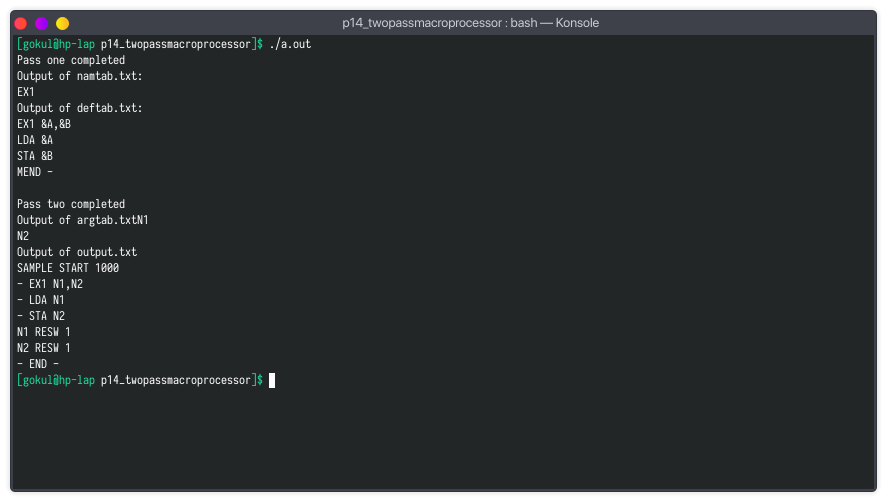
\includegraphics[width=\textwidth]{img/p14.png}
     
\Large
\section*{Result}
\large
Two pass macro processor is implemented and its output is verified
\end{document}